\documentclass[11pt]{article}
\usepackage[margin=1in]{geometry}
\usepackage{booktabs}
\usepackage{graphicx}
\usepackage{pgfplots}
\pgfplotsset{compat=1.17}
\usepackage{float}
\usepackage{caption}
\usepackage{subcaption}
\usepackage{amsmath}
\usepackage{siunitx}
\usepackage{multirow}
\usepackage{cite}
\usepackage[colorlinks=true, linkcolor=blue, urlcolor=blue]{hyperref}

\title{Impact of Simulation Parameters on 3D NeuroSim Performance and Accuracy}
\author{Mohammadhossein Allahakbari}
\date{28/3/2025}

\begin{document}

\maketitle

\begin{abstract}
This report presents the experimental results obtained by varying key simulation parameters in Heterogeneous 3D NeuroSim. A baseline is established by using a VGG-8 model on the CIFAR-10 dataset and default parameters. We then analyze the impact on performance and accuracy when modifying:
\begin{enumerate}
    \item \textbf{Memory Cell Type:} SRAM vs. RRAM.
    \item \textbf{ADC Precision:} Different bit-precisions.
    \item \textbf{ADC Sharing Degree:} Varying the number of columns sharing one ADC.
    \item \textbf{Novel Mapping Parameter:} Enabling/disabling novel weight mapping.
\end{enumerate}
\end{abstract}

\section{Introduction}
3D NeuroSim is used to simulate the hardware performance of neural network accelerators with heterogeneous 3D memory architectures. In the baseline configuration, the simulator was set with:
\begin{itemize}
    \item Memory cell: RRAM
    \item ADC precision: 5 bits
    \item ADC sharing degree: 8 columns per ADC
    \item Novel Mapping: enabled
\end{itemize}
The baseline results and the effects of varying other parameters are discussed in subsequent sections.

\section{Test Setup}
All experiments were performed using a VGG-8 model on the CIFAR-10 dataset. The simulation metrics recorded many metrics but the focus of our study is on the following:
\begin{itemize}
    \item \textbf{Test Accuracy:} Classification accuracy.
    \item \textbf{Hardware Performance:} Layer-by-Layer Read latency, total dynamic energy, and chip area.
    \item \textbf{Throughput:} Layer-by-Layer FPS.
\end{itemize}
Each experiment was run by only changing the parameter in question while leaving all the other parameters identical to the baseline.

\section{Results and Analysis}

\subsection{RRAM vs. SRAM}
This section compares the baseline results to the SRAM results.

\paragraph{Observations:}
\begin{itemize}
    \item \textbf{Test Accuracy:} Both RRAM and SRAM based architectures achieved identical results with 92\% inference accuracy.
    \item \textbf{Latency:} RRAM layer-by-layer read latency is approximately $1.0362\times10^6$ ns, whereas SRAM latency is about $3.0463\times10^6$ ns.
    \item \textbf{Dynamic Energy:} Baseline total read dynamic energy is approximately $1.29545\times10^7$ pJ, compared to $5.34889\times10^7$ pJ in the SRAM run.
    \item \textbf{Throughput:} Baseline yields roughly 965 FPS versus approximately 328 FPS for SRAM.
    \item \textbf{Chip Clock Period and Area:} Baseline clock period is around 1.93 ns, while SRAM operates with a higher clock period (about 4.93 ns) and requires a larger chip area.
\end{itemize}

\subsubsection{Dynamic Energy Comparison}
Figure~\ref{fig:baseline_energy_bar} illustrates the rescaled total read dynamic energy for both configurations (in units of $10^7$ pJ) using a bar chart.

\begin{figure}[H]
    \centering
    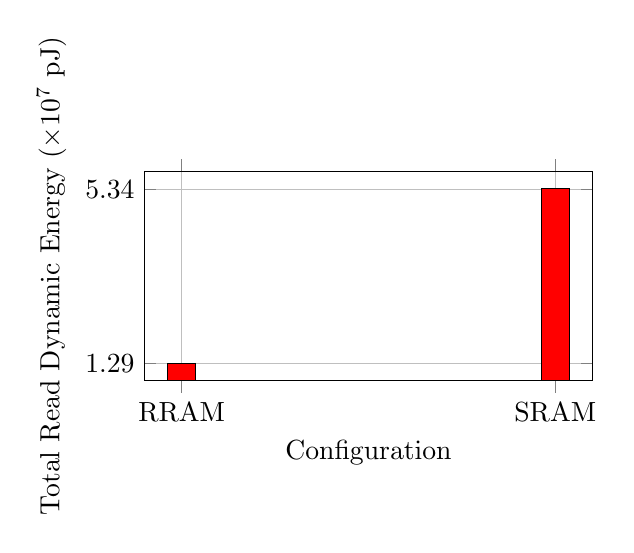
\begin{tikzpicture}
    \begin{axis}[
        ybar,
        xlabel={Configuration},
        ylabel={Total Read Dynamic Energy ($\times10^7$ pJ)},
        symbolic x coords={RRAM, SRAM},
        xtick=data,
        grid=both,
        width=0.6\textwidth,
        height=0.35\textwidth,
        % ymode=log,
        % log basis y={10},
        ytick={1.29, 5.34}
    ]
    \addplot[
        fill=red,
    ]
    coordinates {
        (RRAM,1.29545) (SRAM,5.34889)
    };
    \end{axis}
    \end{tikzpicture}
    \caption{Total read dynamic energy for baseline vs. SRAM configurations.}
    \label{fig:baseline_energy_bar}
\end{figure}


\paragraph{Discussion:}
The comparison shows that the SRAM configuration has significantly higher dynamic energy consumption and increased latency, leading to reduced throughput compared to the baseline.


\subsection{Impact of ADC Precision Variation}
The ADC precision was varied to study its effect on both model accuracy and hardware performance. The baseline configuration uses a 5-bit ADC. Two additional tests were performed using 4-bit and 3-bit ADC precision. Lower ADC resolutions were not experimented with as the accuracy dropped to close to zero values.

\paragraph{Observations:}
\begin{itemize}
    \item \textbf{Test Accuracy:} The 3-bit configuration resulted in extremely low test accuracy (10\%), the 4-bit ADC yielded an intermediate test accuracy of 56\% and the baseline 5-bit configuration achieved 92\% accuracy.
    \item \textbf{Read Latency:} \begin{itemize}
            \item 3-bit ADC: $1.14262\times10^6$ ns
            \item 4-bit ADC: $1.17485\times10^6$ ns
            \item 5-bit ADC: $2.80909e\times10^6$ ns
        \end{itemize}
    \item \textbf{Dynamic Energy:} \begin{itemize}
            \item 3-bit ADC: $2.09866\times10^7$ pJ
            \item 4-bit ADC: $2.46563\times10^7$ pJ
            \item 5-bit ADC: $3.19058\times10^7$ pJ
        \end{itemize}
    \item \textbf{Throughput:} \begin{itemize}
            \item 3-bit ADC: 875.18 FPS
            \item 4-bit ADC: 851.175 FPS
            \item 5-bit ADC: 355.987 FPS
        \end{itemize}
    \item \textbf{Chip Area:} \begin{itemize}
            \item 3-bit ADC: $1.07516\times 10^{-5} ~{mm}^2$
            \item 4-bit ADC: $1.22559\times 10^{-5} ~{mm}^2$
            \item 5-bit ADC: $2.04189\times 10^{-5} ~{mm}^2$
        \end{itemize}
\end{itemize}

\subsubsection{Test Accuracy Comparison}
Figure~\ref{fig:adc_accuracy_line} shows a line graph that compares the test accuracy for the three ADC precision settings.

\begin{figure}[H]
    \centering
    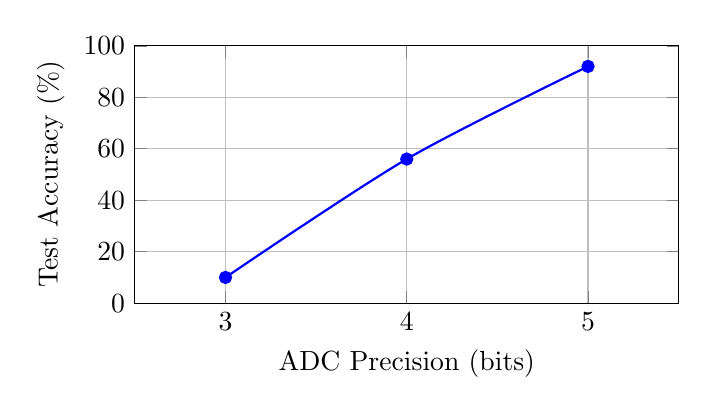
\begin{tikzpicture}
    \begin{axis}[
        xlabel={ADC Precision (bits)},
        ylabel={Test Accuracy (\%)},
        xmin=2.5, xmax=5.5,
        ymin=0, ymax=100,
        xtick={3,4,5},
        grid=both,
        width=0.7\textwidth,
        height=0.4\textwidth,
        smooth
    ]
    \addplot[
        mark=*,
        color=blue,
        thick
    ]
    coordinates {
        (3,10) (4,56) (5,92)
    };
    \end{axis}
    \end{tikzpicture}
    \caption{Test accuracy vs. ADC precision.}
    \label{fig:adc_accuracy_line}
\end{figure}

\subsubsection{Dynamic Energy Comparison}
Figure~\ref{fig:adc_energy_bar} illustrates the rescaled total read dynamic energy (in units of $10^7$ pJ) for each ADC precision test using a bar chart.

\begin{figure}[H]
    \centering
    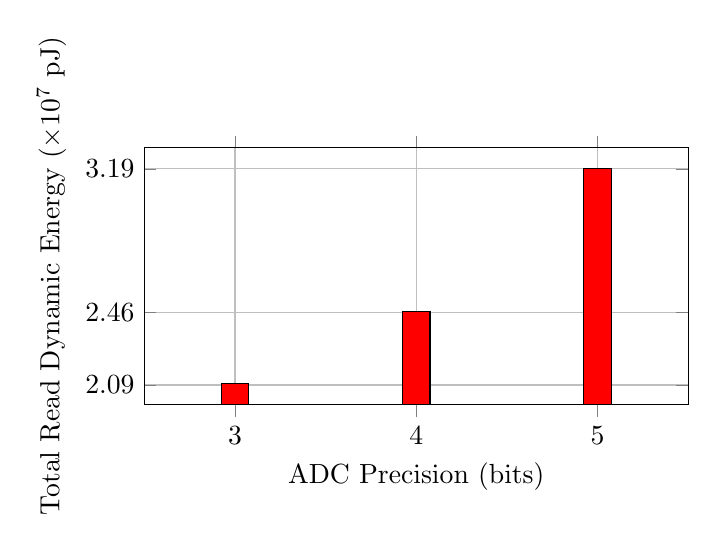
\begin{tikzpicture}
    \begin{axis}[
        ybar,
        xlabel={ADC Precision (bits)},
        ylabel={Total Read Dynamic Energy ($\times10^7$ pJ)},
        xmin=2.5, xmax=5.5,
        xtick={3,4,5},
        grid=both,
        width=0.7\textwidth,
        height=0.4\textwidth,
        % ymode=log,
        % log basis y={10},
        ytick={2.09, 2.46, 3.19}
    ]
    \addplot[
        fill=red,
    ]
    coordinates {
        (3,2.09866) (4,2.46563) (5,3.19058)
    };
    \end{axis}
    \end{tikzpicture}
    \caption{Total read dynamic energy vs. ADC precision.}
    \label{fig:adc_energy_bar}
\end{figure}


\paragraph{Discussion:}
The line charts clearly show that reducing the ADC precision below the baseline (5-bit) negatively impacts the test accuracy while increasing the dynamic energy consumption. In particular, the 3-bit configuration leads to a severe accuracy drop (to 10\%), making it unsuitable for the application. Although the 4-bit configuration performs better than the 3-bit case, it still underperforms compared to the 5-bit setting.

\subsection{Impact of ADC Sharing Degree Variation}
In addition to ADC precision, we investigated the effect of varying the ADC sharing degree. For these experiments, three sharing configurations were tested:
\begin{itemize}
    \item \textbf{8 columns per ADC:} Baseline setting.
    \item \textbf{16 columns per ADC:} Higher sharing degree.
    \item \textbf{32 columns per ADC:} Max sharing degree.
\end{itemize}
\paragraph{Observations:}
\begin{itemize}
    \item \textbf{Test Accuracy:} All different sharing degrees acheived identical results with the accuracy of 92\%, similar to the baseline.
    \item \textbf{Read Latency:} \begin{itemize}
            \item 8-way sharing: $2.80909\times10^6$ ns
            \item 16-way sharing: $1.31549\times10^6$ ns
            \item 32-way sharing: $1.61826\times10^6$ ns
        \end{itemize}
    \item \textbf{Dynamic Energy:} \begin{itemize}
            \item 8-way sharing: $3.19058\times10^7$ pJ
            \item 16-way sharing: $3.95113\times10^7$ pJ
            \item 32-way sharing: $5.87941\times10^7$ pJ
        \end{itemize}
    \item \textbf{Throughput:} \begin{itemize}
            \item 8-way sharing: 355.987 FPS
            \item 16-way sharing: 760.175 FPS
            \item 32-way sharing: 617.949 FPS
        \end{itemize}
    \item \textbf{Chip Area:} \begin{itemize}
            \item 8-way sharing: $2.04189\times10^{-5} ~{mm}^2$
            \item 16-way sharing: $1.25323\times10^{-5} ~{mm}^2$
            \item 32-way sharing: $1.55235e\times10^{-5} ~{mm}^2$
        \end{itemize}
\end{itemize}

\subsubsection{Dynamic Energy Comparison vs. ADC Sharing Degree}
Figure~\ref{fig:sharing_energy_bar} illustrates the rescaled total read dynamic energy (in units of $10^7$ pJ) for the different sharing configurations using a bar chart.

\begin{figure}[H]
    \centering
    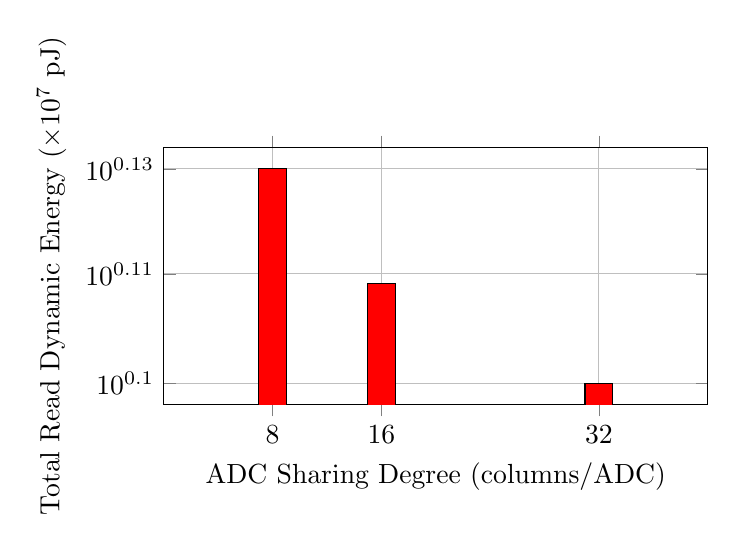
\begin{tikzpicture}
    \begin{axis}[
        ybar,
        xlabel={ADC Sharing Degree (columns/ADC)},
        ylabel={Total Read Dynamic Energy ($\times10^7$ pJ)},
        xmin=0, xmax=40,
        xtick={8,16,32},
        grid=both,
        width=0.7\textwidth,
        height=0.4\textwidth,
        ymode=log,
        log basis y={10},
        ytick={1.25,1.3,1.35}
    ]
    \addplot[
        fill=red,
    ]
    coordinates {
        (8,1.35) (16,1.29545) (32,1.25)
    };
    \end{axis}
    \end{tikzpicture}
    \caption{Total read dynamic energy vs. ADC sharing degree.}
    \label{fig:sharing_energy_bar}
\end{figure}

\paragraph{Discussion:}
The experiments compared ADC sharing configurations of 8, 16, and 32 columns per ADC. All configurations achieved a test accuracy of 92\%. Notably, increasing sharing to 16 columns reduced the read latency from $2.81\times10^6$ ns (8-way) to $1.32\times10^6$ ns and nearly doubled the throughput to 760.175 FPS, albeit with a moderate rise in dynamic energy. In contrast, 32-way sharing slightly increased latency and decreased throughput while further raising energy consumption. Thus, 16-way sharing strikes an optimal balance between latency, energy, throughput, and chip area, as illustrated in Figure \ref{fig:sharing_energy_bar}.


\subsection{Impact of Novel Mapping Parameter} \label{section:mapping_param}
In this section we compare the baseline configuration (with \texttt{novelMapping} enabled) to a run using the conventional mapping method, i.e. with \texttt{novelMapping} disabled. Although both configurations achieve similar test accuracy (around 92\%), there are notable differences in hardware performance.

\paragraph{Observations:}
\begin{itemize}
    \item \textbf{Test Accuracy:} Both configurations achieve approximately 92\% accuracy.
     \item \textbf{Read Latency:} Both configurations achieve identical total read latency of $2.80909\times10^6$ns. 
    \item \textbf{Dynamic Energy:} The baseline configuration (novelMapping enabled) exhibits a total read dynamic energy of about $3.19058\times10^7$ pJ, whereas the non-novel mapping run consumes approximately $3.55067\times10^7$ pJ which is 11\% higher.
    \item \textbf{Throughput:} Both configurations achieve identical throughput of 355.987 FPS
    \item \textbf{Chip Area:} Both configurations require $2.04189e-05 {mm}^2$ of chip area.
\end{itemize}

\subsubsection{Dynamic Energy Comparison: Baseline vs. Non-novel Mapping}
To illustrate the difference in energy consumption, Figure~\ref{fig:novel_mapping_energy_bar} shows a bar chart comparing the rescaled total read dynamic energy (in units of $10^7$ pJ) for the two mapping strategies.

\begin{figure}[H]
    \centering
    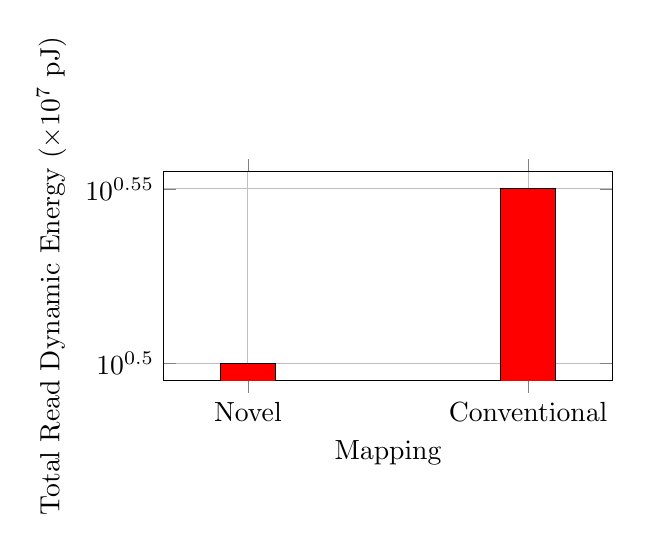
\begin{tikzpicture}
    \begin{axis}[
        ybar,
        bar width=20pt,
        enlarge x limits=0.3,
        xlabel={Mapping},
        ylabel={Total Read Dynamic Energy ($\times10^7$ pJ)},
        symbolic x coords={Novel, Conventional},
        xtick=data,
        grid=both,
        width=0.6\textwidth,
        height=0.35\textwidth,
        ymode=log,
        log basis y={10},
        ytick={3.19, 3.55},
        scaled y ticks=false
    ]
    \addplot[
        fill=red,
    ]
    coordinates {
        (Novel,3.19058) (Conventional,3.55067)
    };
    \end{axis}
    \end{tikzpicture}
    \caption{Total read dynamic energy for baseline (novelMapping enabled) vs. non-novel mapping configurations (rescaled, logarithmic scale).}
    \label{fig:novel_mapping_energy_bar}
\end{figure}



\paragraph{Discussion:}
The bar chart indicates that while both configurations maintain similar test accuracy, the conventional (non-novel) mapping approach results in significantly higher dynamic energy consumption which is tied to the absence of data reuse in this configuration. This, in turn, implies higher latency and reduced throughput. Therefore, enabling the novel mapping parameter leads to improved energy efficiency and overall hardware performance, making it a favorable design choice.

\section{Novel and Conventional Mapping Comparison}
\subsection{Conventional Mapping}
In the conventional mapping approach, each 3D convolution kernel is unrolled into a vertical column, whereby the entire set of weights for a kernel (of dimension K×K×D) is concatenated into a single column within a large weight matrix. This method necessitates that, for every sliding window position during convolution, the same input feature-map (IFM) patch is repeatedly fetched from off-chip buffers and transferred via interconnects to the processing elements. Figure ~\ref{fig:conv_mapping} illustrates how the kernels are unrolled.
\begin{figure}[H]
  \centering
  \includegraphics[width=0.6\textwidth]{asset/conv_map.png} % 
  \caption{Conventional Mapping Scheme.}
  \label{fig:conv_mapping}
\end{figure}


\subsection{Novel Mapping}
The novel mapping technique proposed in \cite{peng2019optimizing} partitions the kernel along its spatial dimensions. Instead of unrolling the entire 3D kernel into a single column, the weights corresponding to each spatial location within the kernel are allocated into separate sub-matrices. Each sub-matrix is then assigned to an individual processing element (PE). Under this scheme, the IFMs are distributed such that each PE receives only the specific input patch pertinent to its corresponding weight block. As the convolution operation advances, the reuse of IFMs is maximized through localized data transfers between adjacent PEs, where only the newly required activations are fetched from the higher-level buffers. Figure \ref{fig:novel_mapping} illustrates how this scheme is implemented.

\begin{figure}[H]
  \centering
  \includegraphics[width=0.7\textwidth]{asset/novel_map.png} % 
  \caption{Novel Mapping Scheme.}
  \label{fig:novel_mapping}
\end{figure}

\subsection{Novel Mapping Benefits}
As illustrated in \ref{section:mapping_param}, this spatially aware partitioning not only minimizes the distance and volume of data movement thereby reducing the latency and energy consumption of interconnects and buffers but also enhances overall system efficiency. The reduction in redundant data transfers leads to a 11\% improvement in energy efficiency (as measured in TOPS/W) for networks such as VGG-8.

\section*{Conclusion}
In summary, our experiments highlight the interplay between accuracy, energy consumption, and hardware performance in 3D NeuroSim under varying simulation parameters. RRAM-based designs offer lower latency, reduced dynamic energy, and higher throughput compared to SRAM, with no accuracy penalty. Increasing ADC precision improves classification accuracy but raises energy use and chip area, with a 5-bit ADC emerging as a practical trade-off. Adjusting the ADC sharing degree indicates that 16 columns per ADC balances energy consumption and throughput more effectively than 8 or 32 columns. Finally, enabling the novel mapping parameter reduces dynamic energy by approximately 11\% while preserving the same accuracy and throughput as conventional mapping. These observations underscore the need for carefully selecting parameters based on the specific performance and efficiency requirements of neuromorphic hardware applications.

\nocite{*}
\bibliographystyle{abbrv}
\bibliography{refrences}

\end{document}